\paragraph{}
Le package RGtk2 s'ajoute en tant que librairie externe pour inclure dans R la possibilité de créer des interfaces graphiques. 

\paragraph{}
Comme dans Explorer3d, on a besoin de gérer les données grâce à l'interface graphique. Cette extension de R est essentielle dans le développement de l'application. 

 \begin{center}
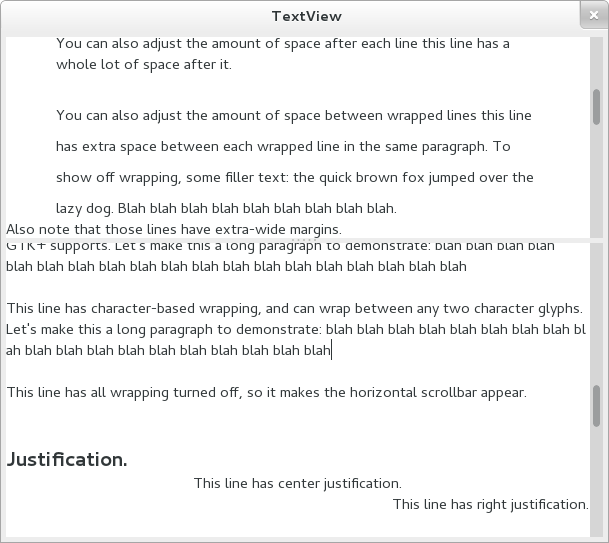
\includegraphics[scale=0.4]{multipleviews.png}\\
\textit{fenêtre divisé en plusieurs parties}
\end{center}

\paragraph{}
RGtk est un package dérivé de GTK2. Il est écrit en c++. GTK est un standart pour la création d'interface utilisateurs en c++ et bien d'autres langages. Grâce à RGtk2 on résout le problème de création d'interface graphique. Comme dans la capture d'écran précédente on peut créer une fenêtre avec plusieurs compartiment à l'intérieur de celle ci. ON peut aussi avoir une fenêtre pour choisir la couleur d'un objet objet affiché dans une vue RGl. 

\begin{center}
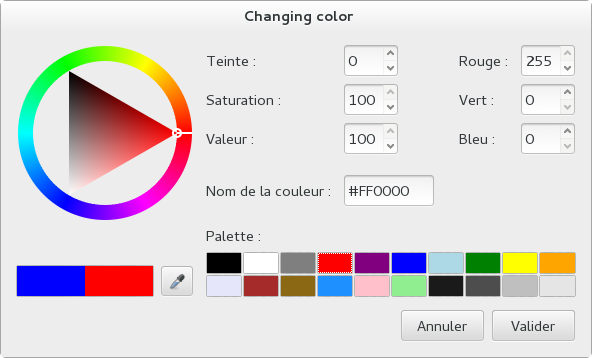
\includegraphics[scale=0.4]{colorselector2.png}
\textit{Selectionneur de couleur RGtk}
\end{center}

\paragraph{}
Le but de RGtk2 est de surcouché GTK. Avec ce package on pourra intéragir avec le logiciel. \\
